% Opcje klasy 'iithesis' opisane sa w komentarzach w pliku klasy. Za ich pomoca
% ustawia sie przede wszystkim jezyk i rodzaj (lic/inz/mgr) pracy, oraz czy na
% drugiej stronie pracy ma byc skladany wzor oswiadczenia o autorskim wykonaniu.
\documentclass[declaration,shortabstract,inz]{iithesis}

\usepackage[utf8]{inputenc}
\usepackage{graphicx}
\graphicspath{{img/}}

%%%%% DANE DO STRONY TYTUŁOWEJ
% Niezaleznie od jezyka pracy wybranego w opcjach klasy, tytul i streszczenie
% pracy nalezy podac zarowno w jezyku polskim, jak i angielskim.
% Pamietaj o madrym (zgodnym z logicznym rozbiorem zdania oraz estetyka) recznym
% zlamaniu wierszy w temacie pracy, zwlaszcza tego w jezyku pracy. Uzyj do tego
% polecenia \fmlinebreak.
\polishtitle    {Badanie gier kooperacyjnych z niepełną\fmlinebreak informacją na przykładzie gry Hanabi}
\englishtitle   {A study on cooperative games with incomplete\fmlinebreak information based on the game of Hanabi}
\polishabstract {\ldots}
\englishabstract{\ldots}
% w pracach wielu autorow nazwiska mozna oddzielic poleceniem \and
\author         {Wojciech Jarząbek \and
				Jacek Leja}
% w przypadku kilku promotorow, lub koniecznosci podania ich afiliacji, linie
% w ponizszym poleceniu mozna zlamac poleceniem \fmlinebreak
\advisor        {dr Paweł Rychlikowski}
%\date          {}                     % Data zlozenia pracy
% Dane do oswiadczenia o autorskim wykonaniu
%\transcriptnum {}                     % Numer indeksu
%\advisorgen    {dr. Pawła Rychlikowskiego} % Nazwisko promotora w dopelniaczu
%%%%%

%%%%% WLASNE DODATKOWE PAKIETY
%
%\usepackage{graphicx,listings,amsmath,amssymb,amsthm,amsfonts,tikz}
%
%%%%% WŁASNE DEFINICJE I POLECENIA
%
%\theoremstyle{definition} \newtheorem{definition}{Definition}[chapter]
%\theoremstyle{remark} \newtheorem{remark}[definition]{Observation}
%\theoremstyle{plain} \newtheorem{theorem}[definition]{Theorem}
%\theoremstyle{plain} \newtheorem{lemma}[definition]{Lemma}
%\renewcommand \qedsymbol {\ensuremath{\square}}
% ...
%%%%%

\begin{document}

\chapter{Wprowadzenie}

\section{Czym jest Hanabi?}

Gry planszowe to forma rozrywki, która towarzyszy człowiekowi od~tysięcy lat. Były one popularne już za~czasów antycznych, czego dowodzi chociażby malowidło z~3300~r.~p.n.e, pochodzące z~grobowca Merknery, na~którym ukazano rozgrywkę Seneta. Przykładem może być także Królewska~Gra~z~Ur, której egzemplarze odnaleziono w~trakcie badań nad~starożytną Mezopotamią. Choć zostały one~w~dzisiejszych czasach w~znacznej mierze zapomniane, nie~sposób nie~wspomnieć o~innych grach z~podobnego okresu, takich~jak~warcaby czy~Go, a~także o~nieco młodszych szachach, które wciąż cieszą~się ogromną i~niesłabnącą popularnością.

Każdą z~tych gier łączy aspekt rywalizacji: pod~koniec rozgrywki jednoznacznie wyszczególnia~się jednego lub~więcej graczy, których określamy mianem zwycięzców, zaś~reszta -~przegrywa. Zgoła inne podejście prezentują gry kooperacyjne, w~których zadaniem nie~jest pokonanie innych uczestników zabawy, a~osiągnięcie wspólnego celu, który gwarantuje wygraną. Można powiedzieć, że~przeciwnikiem graczy jest w~tym przypadku sama gra, która swoją konstrukcją skłania do~współpracy. Co~może zaskakiwać, pierwsze gry tego typu powstały dopiero w~drugiej połowie XX~wieku i~początkowo miały wyłacznie charakter edukacyjny. Wraz z~popularyzacją tzw. "planszówek" gry kooperacyjne w~znacznym stopniu zyskały na~popularności, a~ich forma wyewoluowała w~kierunku zabawy stawiającej na~aspekty towarzyskie, które w~znacznym stopniu ograniczają, lub~wręcz odrzucają współzawodnictwo. Przykładami takiego podejścia mogą~być Pandemic, Martwa Zima, a~także Hanabi, na~którym skupia~się nasza praca.

Hanabi (jap. fajerwerki) to~w~pełni kooperacyjna gra planszowa, która w~2013 roku wygrała prestiżową nagrodę Spiel~des~Jahres. Gracze wcielają~się w~niej w pracowników fabryki fajerwerków, w~której to~pomieszane zostały rodzaje prochu. Celem jest złożenie w~odpowiedniej kolejności możliwie jak~największej ilości sztucznych ogni, które gracze otrzymują poprzez dobieranie kart z~potasowanej talii. Uczestnicy rozgrywki widzą karty, które są~w~posiadaniu innych graczy, lecz~nie~mogą przypatrywać~się~tym, którymi sami dysponują. Dodatkowo, komunikacja odnosząca~się do~treści kart podlega restrykcyjnym zasadom i~jest w~znacznym stopniu ograniczona, co~w~oczywisty sposób czyni rozgrywkę niebanalną. Jakie strategie należy zatem zastosować, by~wygrać? Jak można przełożyć je~na~świat algorytmów?

\section{Hanabi a sztuczna inteligencja}

W~teorii gier istnieje pojęcie perfekcyjnego zagrania, czyli pojedynczego ruchu zależnego od~aktualnego etapu gry, który prowadzi do~stanu rozgrywki maksymalizującego oczekiwany wynik, niezależnie od~ruchów, które mogą w~odpowiedzi wykonać inni gracze. Perfekcyjne zagrania są~podstawą optymalnego planu działania, który minimalizuje możliwe straty ponoszone w~trakcie rozgrywania danej partii. Niestety, tak~silna strategia w~przypadku złożonych gier jest nieprawdopodobnie trudna do~uzyskania ze~względu na~ogromną rozpiętość drzewa możliwych do~uzyskania stanów rozgrywki. W~praktyce używa~się algorytmów: heurystycznych, regułowych, opartych na~technikach uczących, nadużywających zasad gry lub~siłowych. Przykładowo, słynny komputer Deep Blue, który w~maju 1997 roku pokonał ówczesnego mistrza świata w~szachach, Garrego Kasparova, nie~posiadał optymalnej strategii. Używał on~w~zamian metody siłowej, wspomaganej algorytmem przeszukującym alfa-beta, rozpatrując wszystkie możliwe zagrania i~wybierając~te, które dawały mu~największą przewagę lokalną. Takie podejście było możliwe z~racji na ogromną moc superkomputera, który potrafił rozpatrywać 200~milionów ruchów na~sekundę.

Stworzenie sztucznej inteligencji do~Hanabi to~zadanie, które wymaga pokonania trudności niespotykanych w~innych grach. Jest to~następstwo kilku czynników: niepełnej informacji, losowości dobieranych kart, a~także ograniczonych zasobów, m.in. w~postaci podpowiedzi dla~innych graczy. Agenci muszą sobie ufać, gdyż gracz, który nie~chce współpracować, może w~kilku ruchach doprowadzić do~przegranej całej grupy. Ważne jest, by~nie~marnować zasobów, a~zatem sztuczna inteligencja musi być odpowiednio skoordynowana z~innymi graczami. Ponadto, znikoma ilość kart w~talii nie~pozwala na~wygraną w sytuacji, w~której zagrywane są~wyłącznie karty z~pełną informacją. Oznacza to~zatem, że~agenci muszą posiadać protokół komunikacji, który pozwala im~na~przekazywanie w~obrębie zasad gry dodatkowych, implicytnych informacji, rozumianych przez pozostałych jej~uczestników.

Niniejsza praca ma~na~celu zbadanie Hanabi jako gry kooperacyjnej z~niepełną informacją. Przedstawimy techniki tworzenia agentów sztucznej inteligencji grających w~Hanabi, którzy wykonują możliwie najbardziej efektywne i zrozumiałe dla ludzi ruchy na~tyle szybko, by~umożliwić komfortową rozgrywkę z~człowiekiem na~zwykłych komputerach.


\chapter{Zasady gry}

\renewcommand{\thefigure}{1}
\begin{figure}[ht!]
	\centering
	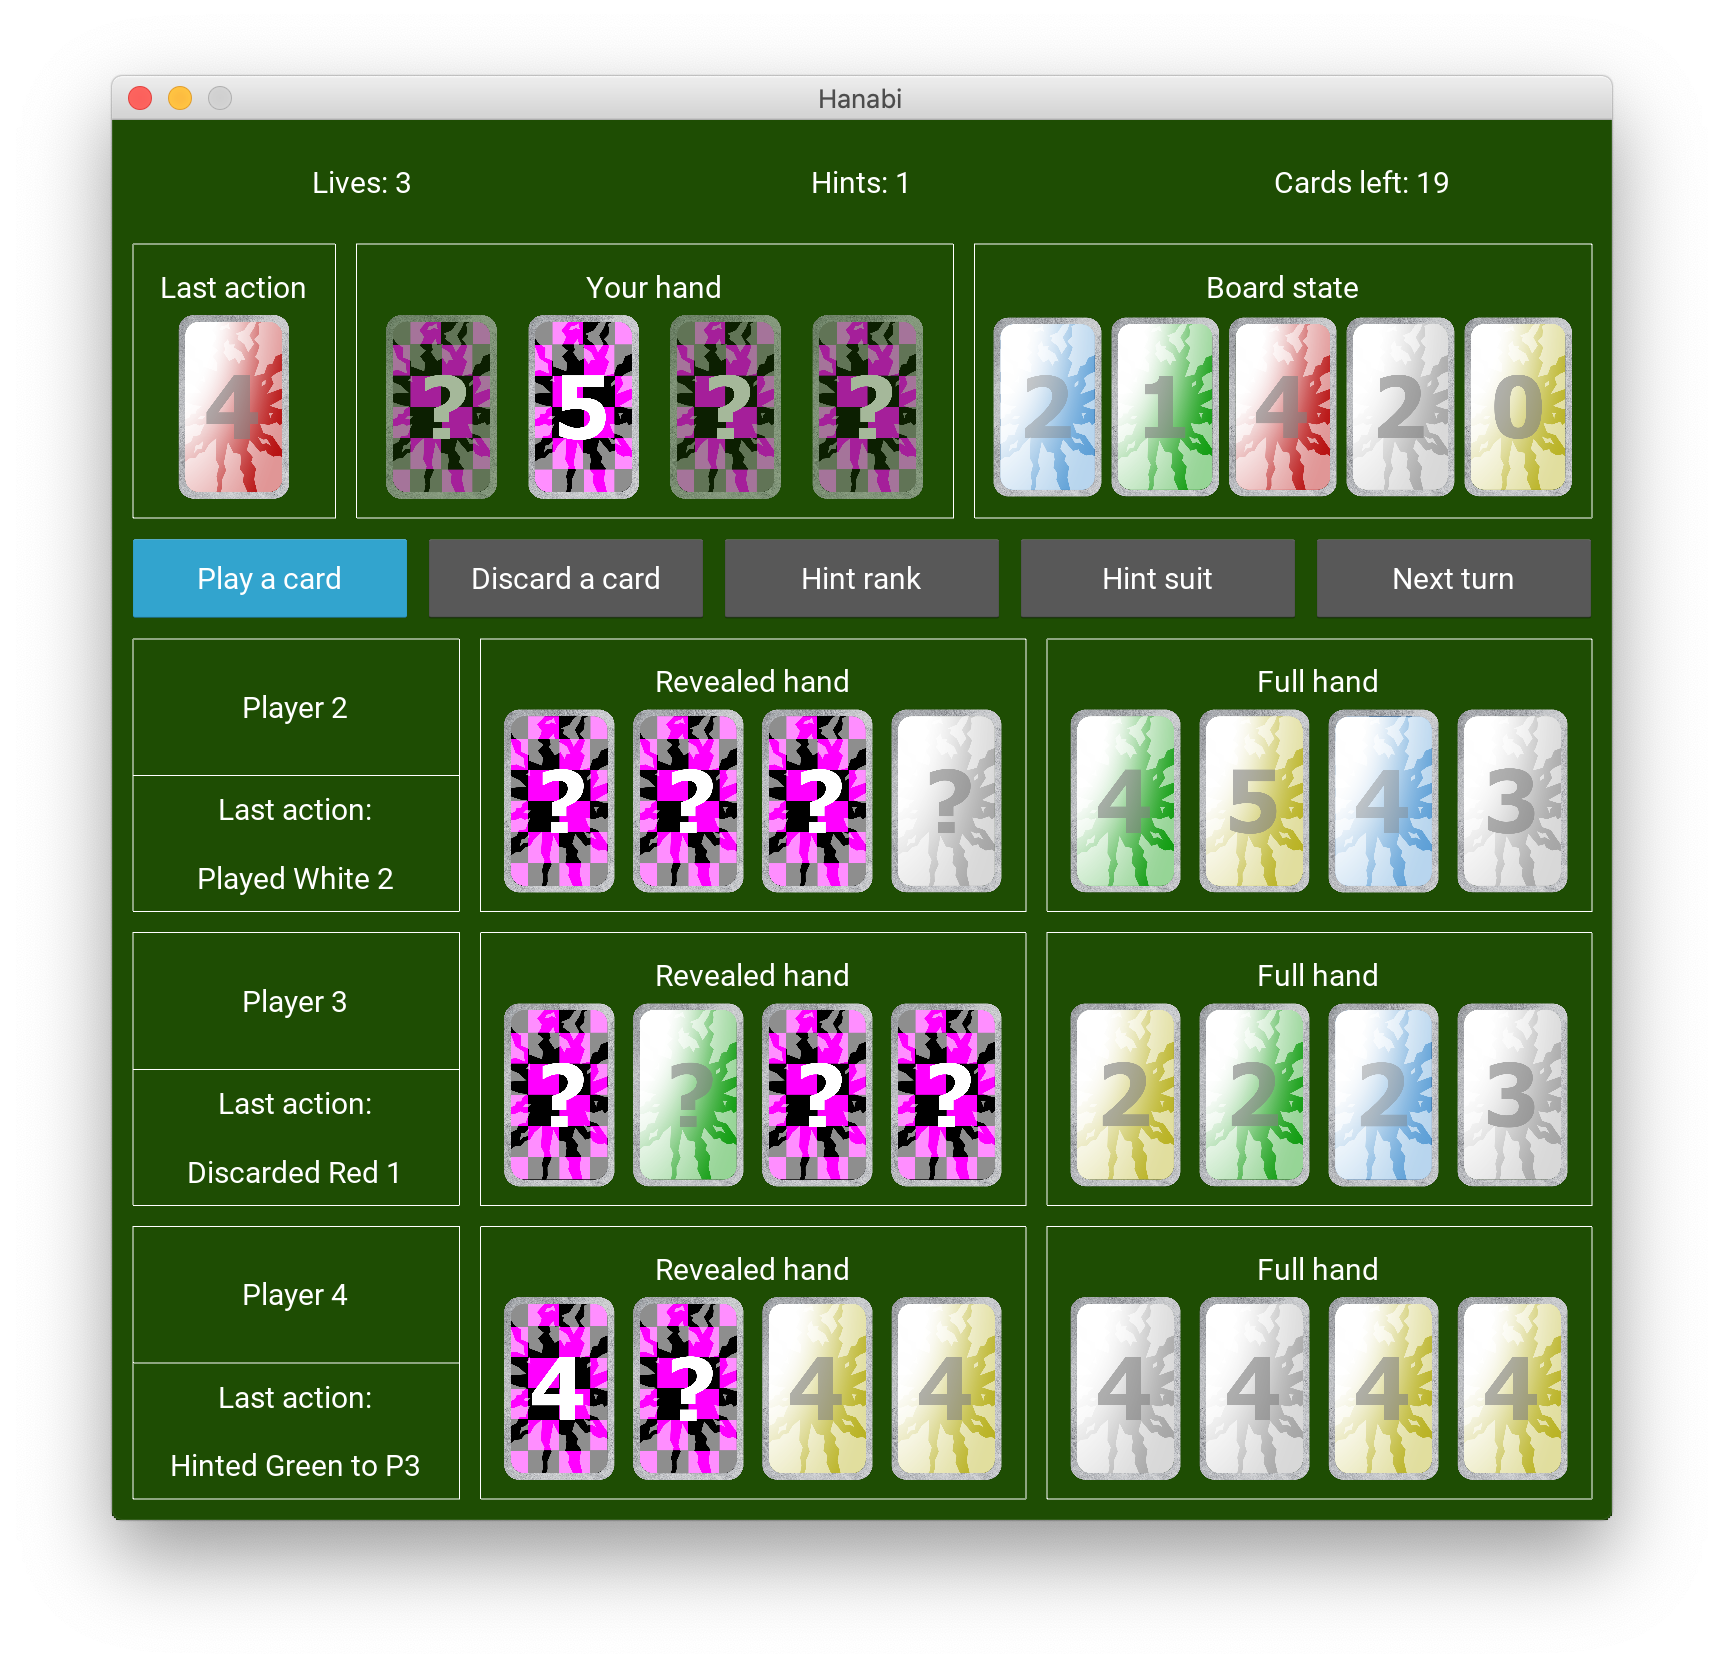
\includegraphics[width=1.0\linewidth]{gui.png}
	\caption[Caption]{Interfejs graficzny do gry Hanabi}
\end{figure}

\newpage

\section{Wyjaśnienie zasad}

Talia do~gry składa~się z~pięćdziesięciu kart. Każda karta jest~oznaczona jednym z~pięciu kolorów (czerwony, żółty, niebieski, biały, zielony) oraz jedną z~wartości z~zakresu od~1~do~5. Dla każdego koloru istnieją po~trzy karty o~numerze~1, po~dwie karty o~numerach 2,~3~i~4, a~także po~jednej karcie o~numerze~5.

Na początku gry talia jest tasowana. Gracze rozpoczynają rozgrywkę z~ośmioma żetonami podpowiedzi i~trzema żetonami życia. Żetony te są wspólne dla wszystkich uczestników rozgrywki. Jeżeli graczy jest dwóch lub~trzech, każdy z~nich dobiera po~cztery zakryte karty. Jeżeli jest ich~czterech lub~pięciu, dobierają po~pięć zakrytych kart. Następnie gracze po kolei wykonują swoje ruchy. Ruch to~wykonanie jednej z~trzech dostępnych akcji (tury~nie~można~pominąć):
\begin{enumerate}
	\item Zagranie karty:

	Gracz deklaruje chęć zagrania karty, wybiera zakrytą kartę ze swojej ręki, a~następnie wykłada ją~na~stół w~pozycji odkrytej. Karty muszą być~zagrywane w~kolejności rosnącej, zaczynając od~jedynki, inaczej zagranie uważa~się za~niepoprawne. Przykładowo, jeśli na~stole~nie ma~żadnych kart, można zagrać tylko te~oznaczone numerem~1. Jeżeli na~stole znajduje~się wyłącznie niebieska karta o~numerze~1 i~żółta karta o~numerze~4, można zagrać niebieską kartę o~numerze~2, żółtą kartę o~numerze~5, lub dowolną kartę innego koloru o~numerze~1. Jeżeli karta została zagrana poprawnie, jest ona dodawana do~stosu o~odpowiednim kolorze, lub~też~rozpoczyna stos swojego koloru. Jeżeli karta została zagrana niepoprawnie, jest ona~usuwana z~gry, a~gracze tracą jeden z~żetonów życia. Dodatkowo, jeżeli zagrana karta ma~numer~5, gracze otrzymują jeden żeton podpowiedzi (chyba, że~mają ich już osiem). Po~rozpatrzeniu efektów akcji gracz dobiera zakrytą kartę z~talii (jeżeli nie~jest ona~pusta).
	
	\item Odrzucenie karty:
 
	Gracz deklaruje chęć odrzucenia karty, wybiera zakrytą kartę ze swojej ręki, a~następnie wykłada ją~na~stół w~pozycji odkrytej. Karta ta~jest usuwana z~gry, bez dokładania do~któregokolwiek ze~stosów, a~gracze otrzymują jeden żeton podpowiedzi, jeżeli aktualna ilość żetonów podpowiedzi jest~mniejsza niż~osiem. W~przeciwnym wypadku odrzucenie karty nie~ma~żadnego dodatkowego efektu. Po~rozpatrzeniu efektów akcji gracz dobiera zakrytą kartę z~talii (jeżeli nie~jest ona~pusta).

	\item Udzielenie podpowiedzi innemu graczowi:

	Gracz usuwa jeden z~żetonów podpowiedzi, wybiera innego uczestnika rozgrywki, a~następnie może udzielić mu~jednej z~dwóch informacji: wskazać wszystkie jego karty o~wybranym kolorze, lub~wszystkie jego karty o~wybranym numerze. Akcji tej nie~można wykonać, jeśli w~grze~nie ma~żadnych żetonów podpowiedzi.
\end{enumerate}

Jeżeli któryś z graczy dobierze ostatnią kartę z~talii, każdy uczestnik rozgrywa jedną dodatkową turę (wraz z~graczem, który dobrał ostatnią kartę), po~czym gra~się kończy.

Gra natychmiast kończy~się, gdy~zostanie utracony ostatni żeton życia, lub gdy~wszystkie stosy odpowiednich kolorów zostały skompletowane (na~każdy z~nich położono kartę o~numerze~5).

Po~zakończeniu gry ilość uzyskanych punktów oblicza~się poprzez zsumowanie wartości najwyższych kart z~każdego ze~stosów odpowiedniego koloru, można zatem uzyskać maksymalnie dwadzieścia pięć punktów.

\section{Niepisane obserwacje}

\ldots

%%%%% BIBLIOGRAFIA

%\begin{thebibliography}{1}
%\bibitem{example} \ldots
%\end{thebibliography}

\end{document}
